\documentclass[11pt, a4paper]{jarticle}

% 数式
\usepackage{amsmath,amsfonts}
\usepackage{bm}
% 画像
\usepackage{graphicx}
\usepackage[dvipdfmx]{color}

\usepackage[margin=15mm]{geometry}
\usepackage{float}
\usepackage{siunitx}

\usepackage{tikz}
\usetikzlibrary{automata, positioning}

\usepackage{url}

% \usepackage{algorithm}
% \usepackage{algpseudocode}
\usepackage[linesnumbered,ruled,vlined]{algorithm2e}


\title{データセンタにおける光回線交換ネットワークの設計問題}
\author{緒方雄大}

\begin{document}
\maketitle

\section{知識}
\noindent ・Folded Clos networkではTxとRxのペアがinput-outputレイヤの共通のスイッチに繋がる.\\
・データセンターはUnfolded ClosよりFolded Closを採用.
→全てのスイッチがコンパクトにまとまり、ケーブル長が短くなる. 収容ラックの効率的な使用. Folded Closのほうがスケーラブル\\
・Strict-sense non blocking: \\
・TF Closはinput-ouputスイッチでのポート数の制限を緩和. \\ 

\section{3構成(2TF, 2F, 3UF)でのSwitching capacityの最大化}
\noindent スイッチのポート数$N=64$\\
スイッチ数$a=100$\\
Input-Outputスイッチでのポート数$n$\\
Input-Outputスイッチ数$k$\\
Intermediateスイッチ数$m$\\
Input-OutputスイッチとIntermediateスイッチ間のリンク数$v$

\subsection{Two-stage twisted and folded Clos network (2TF)}

\begin{figure}[H]
    \centering
    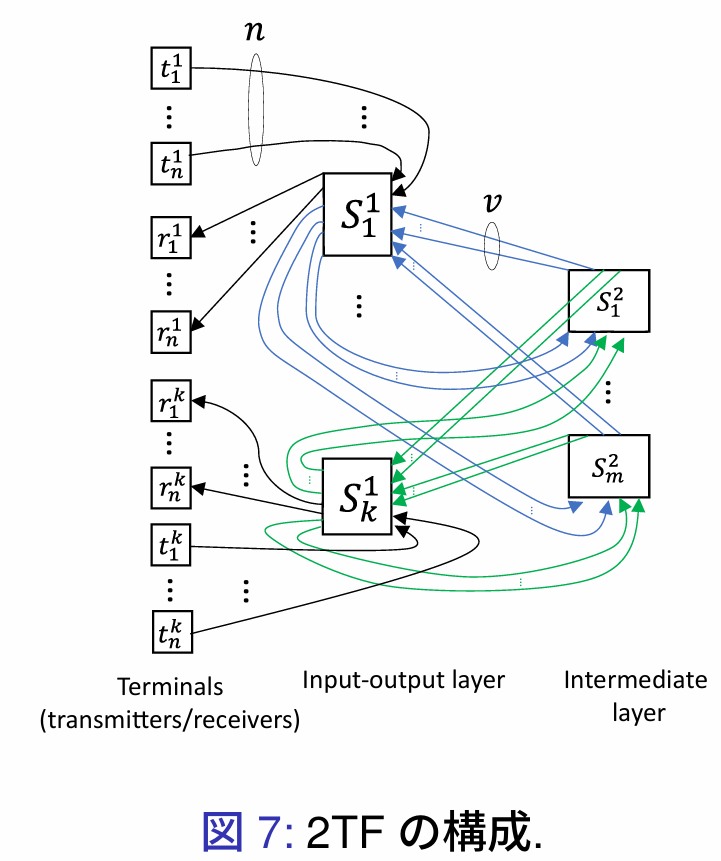
\includegraphics[width=0.5\linewidth]{2tf.png}
  \end{figure}

\begin{align}
    & \max  &n \cdot k \\
    & \text{s.t.} & n + v m \leq N \\
    && v k \leq N \\
    && 2 \left\lfloor \frac{n-1}{v} \right\rfloor + 1 &\leq m \\
    && k + m \leq a\\
\end{align}

\begin{algorithm}[H]
    \caption{2TFでの$n \cdot k$の最大化アルゴリズム}
    \KwIn{$N = 64$, $a = 100$}
    \KwOut{max $n \cdot k$ と対応する $(n, k, m, v)$}
    $max\_nk \gets 0$, $best\_params \gets \text{None}$\;
    \For{$n \gets 1$ \KwTo $N$}{
      \For{$k \gets 1$ \KwTo $a$}{
        $nk \gets n \cdot k$\;
        \If{$nk \leq max\_nk$}{
          \textbf{continue}\;
        }
        \For{$v \gets 1$ \KwTo $a$}{
          \If{$v \cdot k > N$}{
            \textbf{break}\;
          }
          \For{$m \gets 1$ \KwTo $a$}{
            \If{$k + m > a$}{
              \textbf{break}\;
            }
            \If{$n + v \cdot m > N$}{
              \textbf{break}\;
            }
            \If{$2 \cdot \left\lfloor \dfrac{n - 1}{v} \right\rfloor + 1 \leq m$}{
              \If{$nk > max\_nk$}{
                $max\_nk \gets nk$\;
                $best\_params \gets (n, k, m, v)$\;
              }
            }
          }
        }
      }
    }
    \Return $max\_nk$, $best\_params$\;
\end{algorithm}

・$(n, k, m, v) = (21, 59, 41, 1)$のとき, $$nk=1239$$

\subsection{Two-stage folded Clos network (2F)}

\begin{figure}[H]
    \centering
    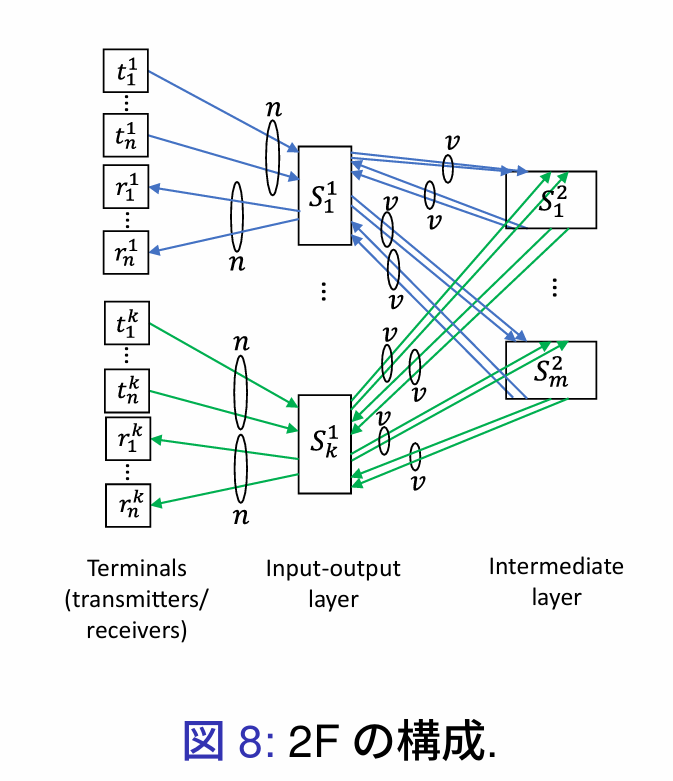
\includegraphics[width=0.5\linewidth]{2f.png}
    % \caption{滞在時間のヒストグラム}
    % \label{fig:histogram}
  \end{figure}

\begin{align}
    & \max  &n \cdot k \\
    & \text{s.t.} & 2n \leq N \\
    && 2 v m \leq N\\
    && v k \leq N \\
    && 2 \left\lfloor \frac{n-1}{v} \right\rfloor + 1 &\leq m \\
    && k + m \leq a\\
\end{align}

\begin{algorithm}[H]
    \caption{2Fでの$n \cdot k$の最大化アルゴリズム}
    \KwIn{$N = 64$, $a = 100$}
    \KwOut{max $n \cdot k$ と対応する $(n, k, m, v)$}
    $max\_nk \gets 0$, $best\_params \gets \text{None}$\;
    \For{$n \gets 1$ \KwTo $N/2$}{
      \For{$k \gets 1$ \KwTo $a$}{
        $nk \gets n \cdot k$\;
        \If{$nk \leq max\_nk$}{
          \textbf{continue}\;
        }
        \For{$v \gets 1$ \KwTo $a$}{
          \If{$v \cdot k > N$}{
            \textbf{break}\;
          }
          \For{$m \gets 1$ \KwTo $a$}{
            \If{$k + m > a$}{
              \textbf{break}\;
            }
            \If{$2 \cdot v \cdot m > N$}{
              \textbf{break}\;
            }
            \If{$2 \cdot \left\lfloor \dfrac{n - 1}{v} \right\rfloor + 1 \leq m$}{
              \If{$nk > max\_nk$}{
                $max\_nk \gets nk$\;
                $best\_params \gets (n, k, m, v)$\;
              }
            }
          }
        }
      }
    }
    \Return $max\_nk$, $best\_params$\;
\end{algorithm}

・$(n, k, m, v) = (16, 64, 31, 1)$のとき, $$nk=1024$$

\subsection{Three-stage unfolded Clos network (3UF)}

\begin{figure}[H]
    \centering
    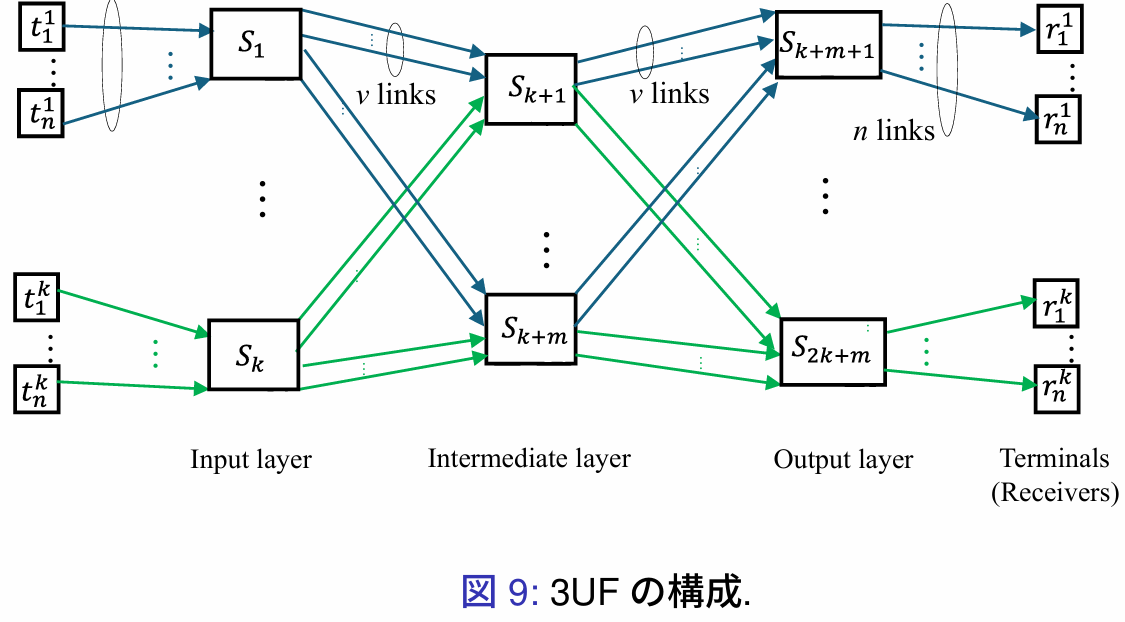
\includegraphics[width=0.5\linewidth]{3uf.png}
    % \caption{滞在時間のヒストグラム}
    % \label{fig:histogram}
\end{figure}

\begin{align}
    & \max  &n \cdot k \\
    & \text{s.t.} & n \leq N \\
    && v m \leq N\\
    && v k \leq N \\
    && 2 \left\lfloor \frac{n-1}{v} \right\rfloor + 1 &\leq m \\
    && 2k + m \leq a\\
\end{align}

\begin{algorithm}[H]
    \caption{3UFでの$n \cdot k$の最大化アルゴリズム}
    \KwIn{$N = 64$, $a = 100$}
    \KwOut{max $n \cdot k$ と対応する $(n, k, m, v)$}
    $max\_nk \gets 0$, $best\_params \gets \text{None}$\;
    \For{$n \gets 1$ \KwTo $N$}{
      \For{$k \gets 1$ \KwTo $a$}{
        $nk \gets n \cdot k$\;
        \If{$nk \leq max\_nk$}{
          \textbf{continue}\;
        }
        \For{$v \gets 1$ \KwTo $a$}{
          \If{$v \cdot k > N$}{
            \textbf{break}\;
          }
          \For{$m \gets 1$ \KwTo $a$}{
            \If{$v \cdot m > N$ \textbf{or} $k + m > a$}{
              \textbf{break}\;
            }
            \If{$2 \cdot \left\lfloor \dfrac{n - 1}{v} \right\rfloor + 1 \leq m$}{
              \If{$nk > max\_nk$}{
                $max\_nk \gets nk$\;
                $best\_params \gets (n, k, m, v)$\;
              }
            }
          }
        }
      }
    }
    \Return $max\_nk$, $best\_params$\;
\end{algorithm}


・$(n, k, m, v) = (32, 32, 31, 2)$のとき, $$nk=1024$$

\subsection{結果}
\noindent 2TF, 2F, 3UFの構成のスイッチングネットワーク$nk$の大小関係は, ($N-64$, $a=100$)\\
2TF(1239) $>$ 2F(1024) $=$ 3UF(1024)

\section{Theorems(Mano論文[1])}
Theorem 1: 2Fのスイッチング容量$f_{2F}(a; N)$と2TFのスイッチング容量$f_{3UF}(a; N)$について, \\
$$f_{2F}(a; N) \leq f_{2TF}(a; N)$$

Theorem 2: 次の条件が成り立つならば, $$f_{3UF}(a; N) \leq f_{2TF}(a; N)$$ \\
条件: 
\begin{align}
    &N \not\equiv 3 \pmod{6} \text{ and } N > 10\\
    &a \leq \frac{4}{\sqrt{3}}(N-1)-1\\
    & f_{3UF}(a; N) > 10N
\end{align}

Theorem 4: if $N > 120$ and $\frac{5N-1}{3} \leq a $, 
$$f_{2TF}(a; N) > 1.3f_{2F}(a; N)$$

Theorem 5: if $N > 40$ and $\frac{5N-1}{3} \leq a \leq 2N-3$, 
$$f_{2TF}(a; N) > 1.3f_{3UF}(a; N)$$


\section{スイッチング数の変更}
\subsection{2TFと3UF}
・$N=32, 64, 128, 256$で$a$を変化させてスイッチングサイズを比較した(全て$N \not\equiv 3 \pmod{6} \text{ and } N > 10$). 
\begin{figure}[H]
    \centering
    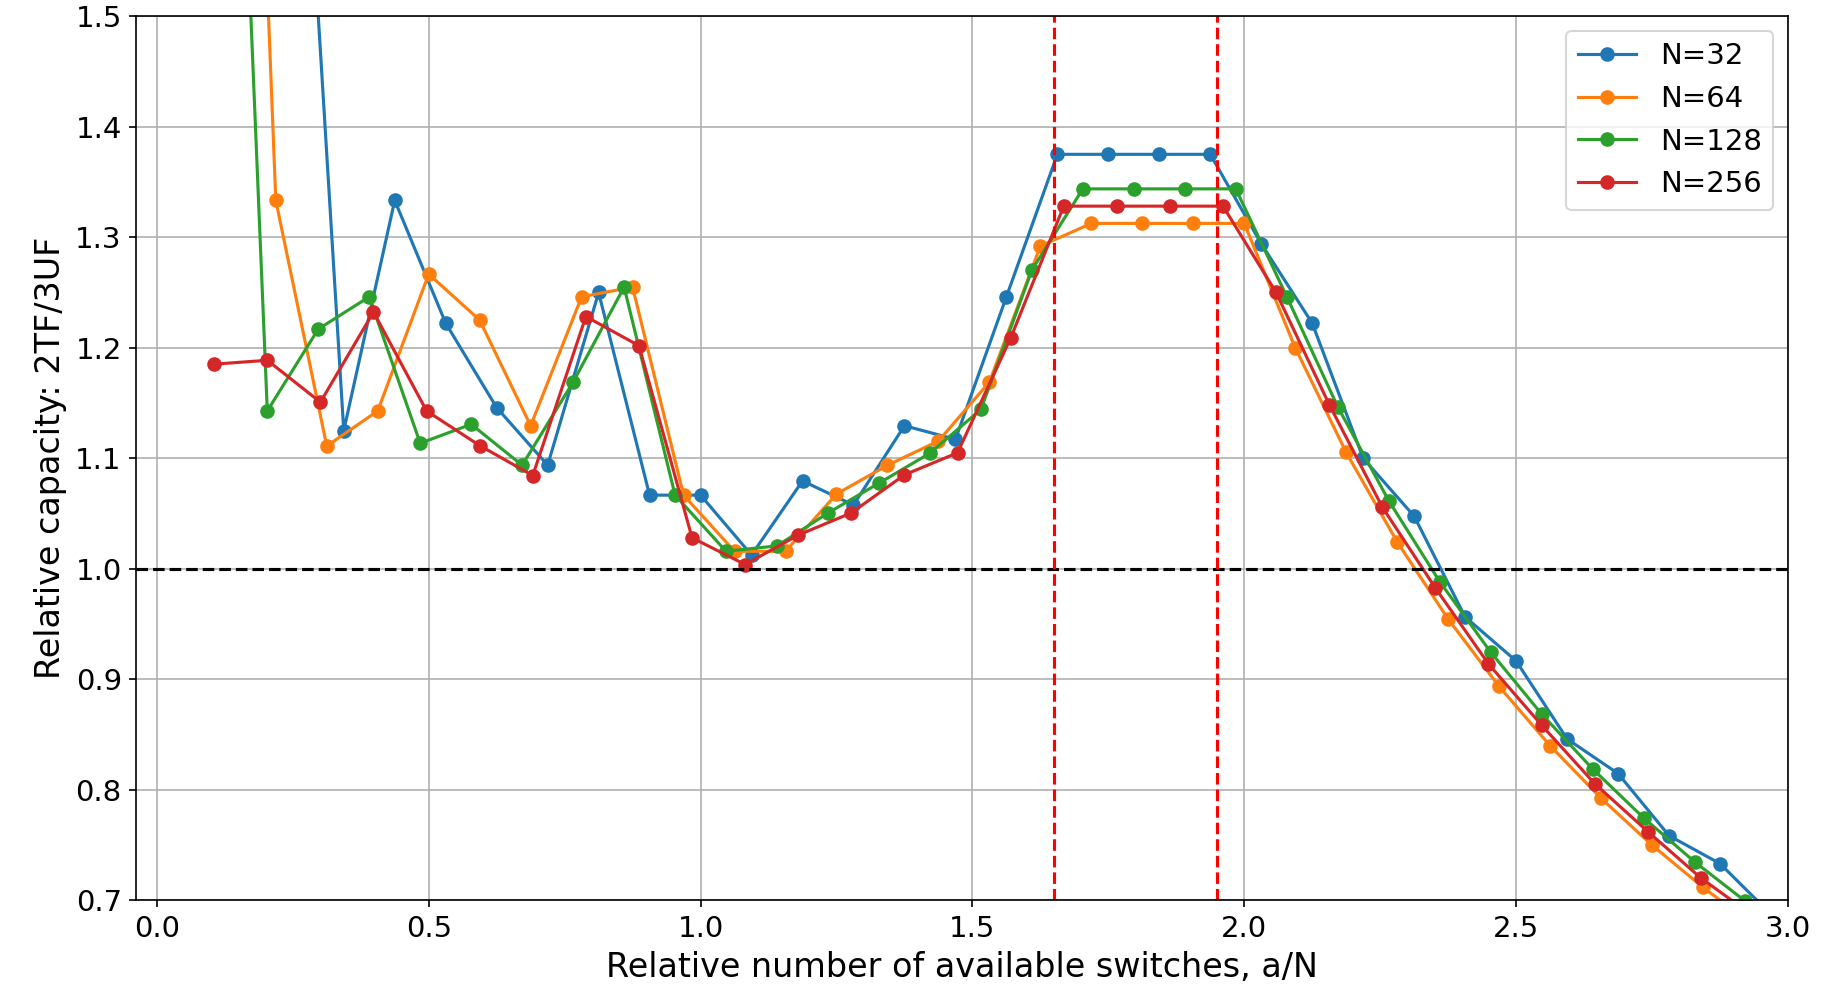
\includegraphics[width=0.8\linewidth]{compare_relative_3uf_1.png}
\end{figure}


・$N=33, 63, 129, 255$で$a$を変化させてスイッチングサイズを比較した(全て$N \equiv 3 \pmod{6} \text{ and } N > 10$).
\begin{figure}[H]
  \centering
  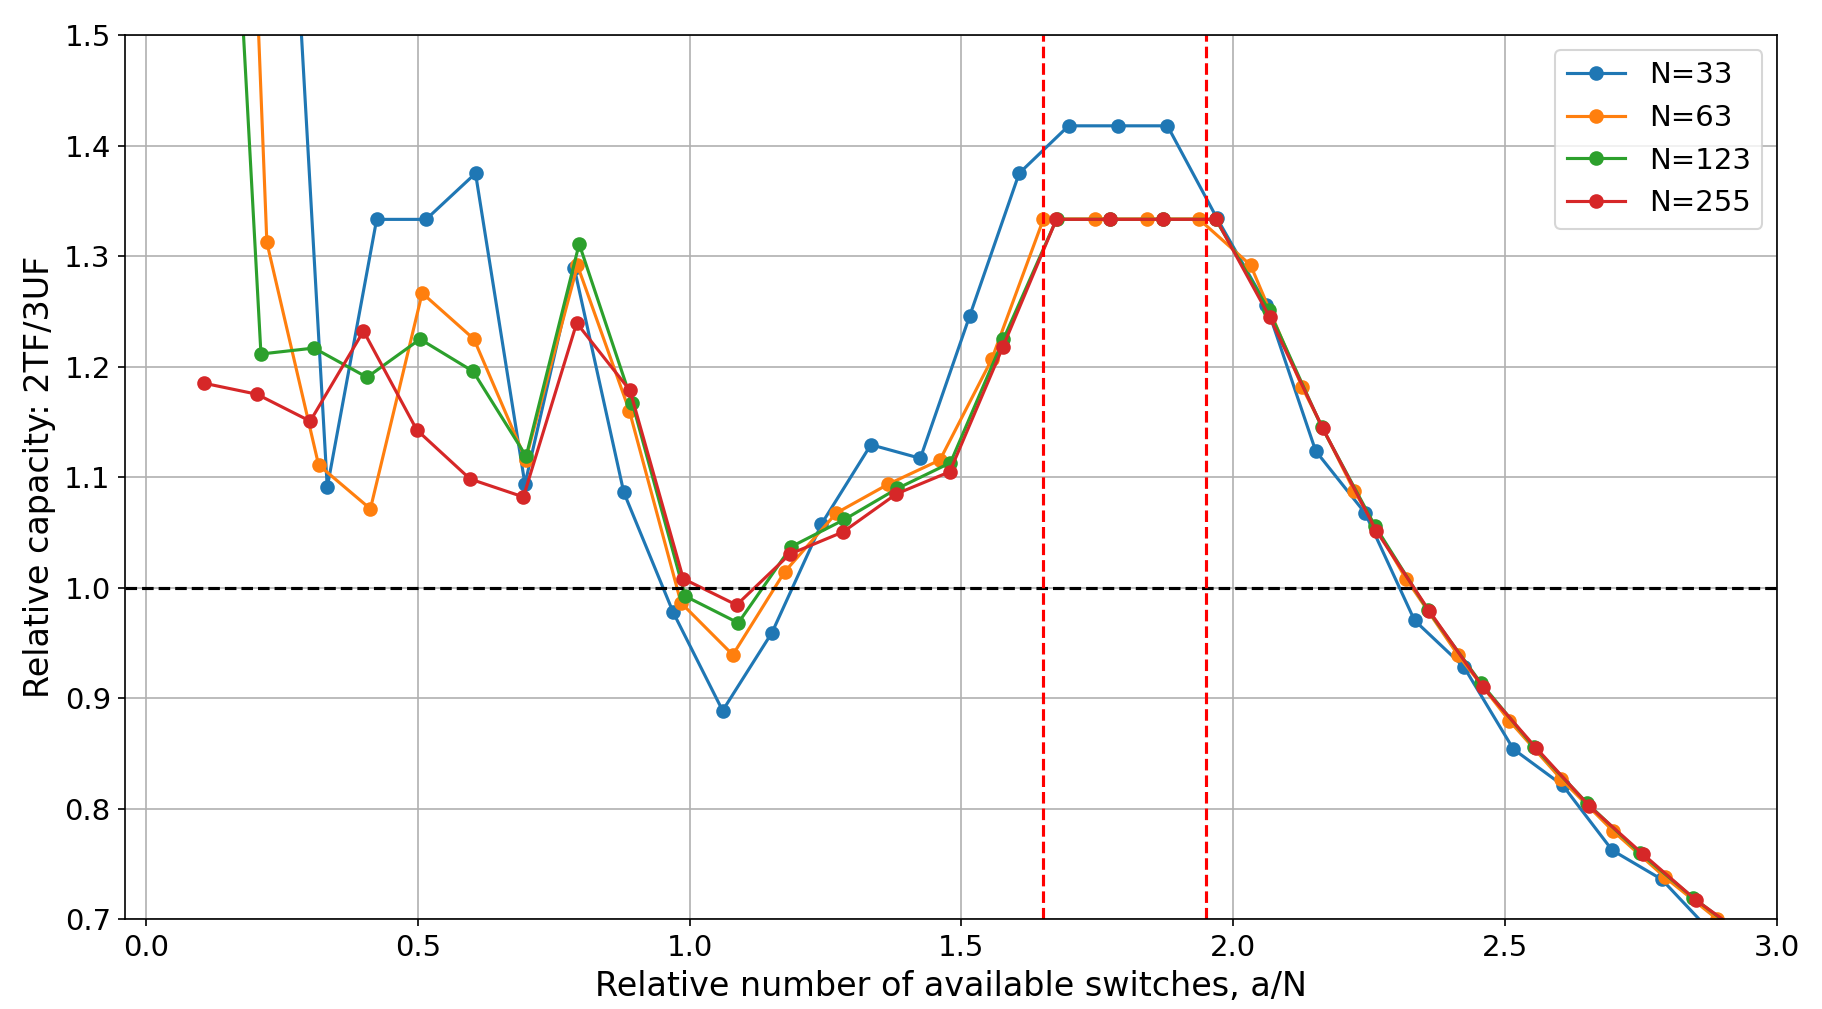
\includegraphics[width=0.8\linewidth]{compare_relative_3uf_2.png}
\end{figure}

\noindent・Theorem 5について, $N=64, 128, 256$($N>40$)のとき, $1.66 \leq \frac{a}{N} \leq 1.95$であれば, $f_{2TF}(a; N) > 1.3f_{3UF}(a; N)$を満たすはず. 
実際にグラフより, この区間で$30\%$以上の増加が見られた(赤のライン).\\
・$N \equiv 3 \pmod{6}$のとき, 下のグラフより, $f_{3UF}(a; N) > f_{2TF}(a; N)$のときがあった(y=1のラインを下回る). これはTheorem 2の条件を満たしていないからである. 
→Capacity Reversing

\subsection{2TFと2F}
・$N=32, 64, 128, 256$で$a$を変化させてスイッチングサイズを比較した. 
\begin{figure}[H]
  \centering
  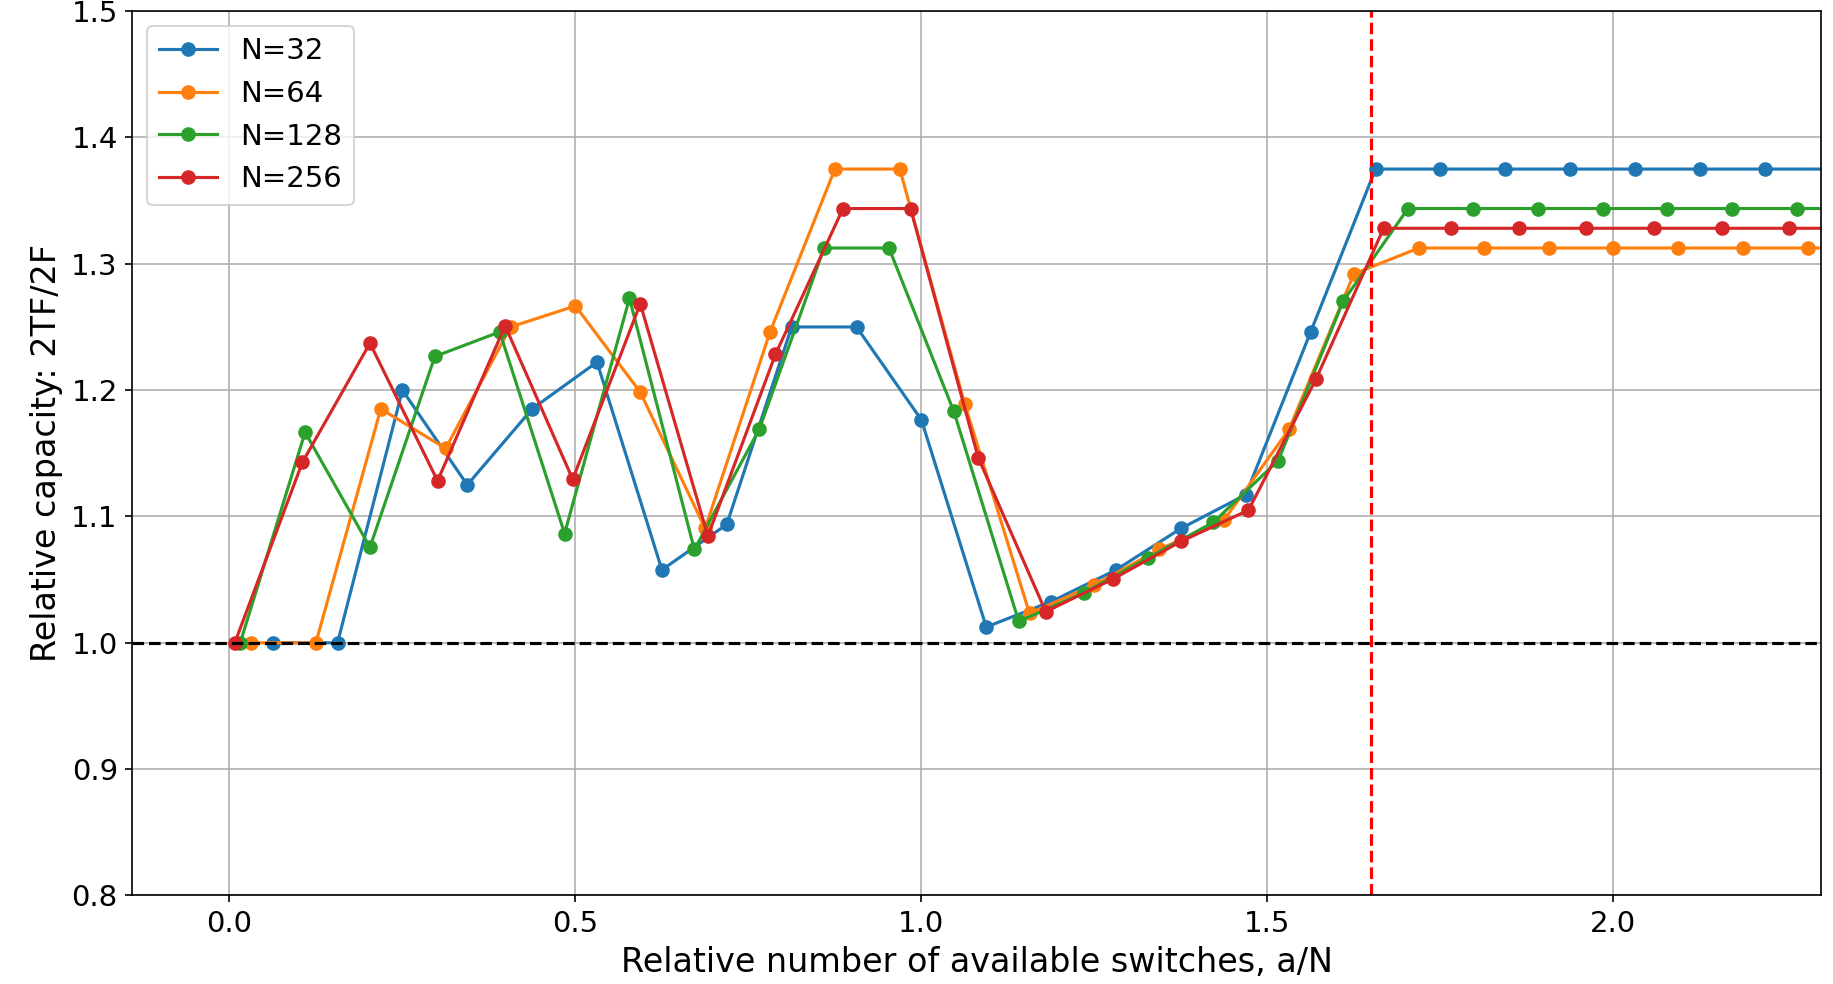
\includegraphics[width=0.8\linewidth]{compare_relative_2f_1.png}
\end{figure}

・$N=33, 63, 129, 255$で$a$を変化させてスイッチングサイズを比較した.
\begin{figure}[H]
  \centering
  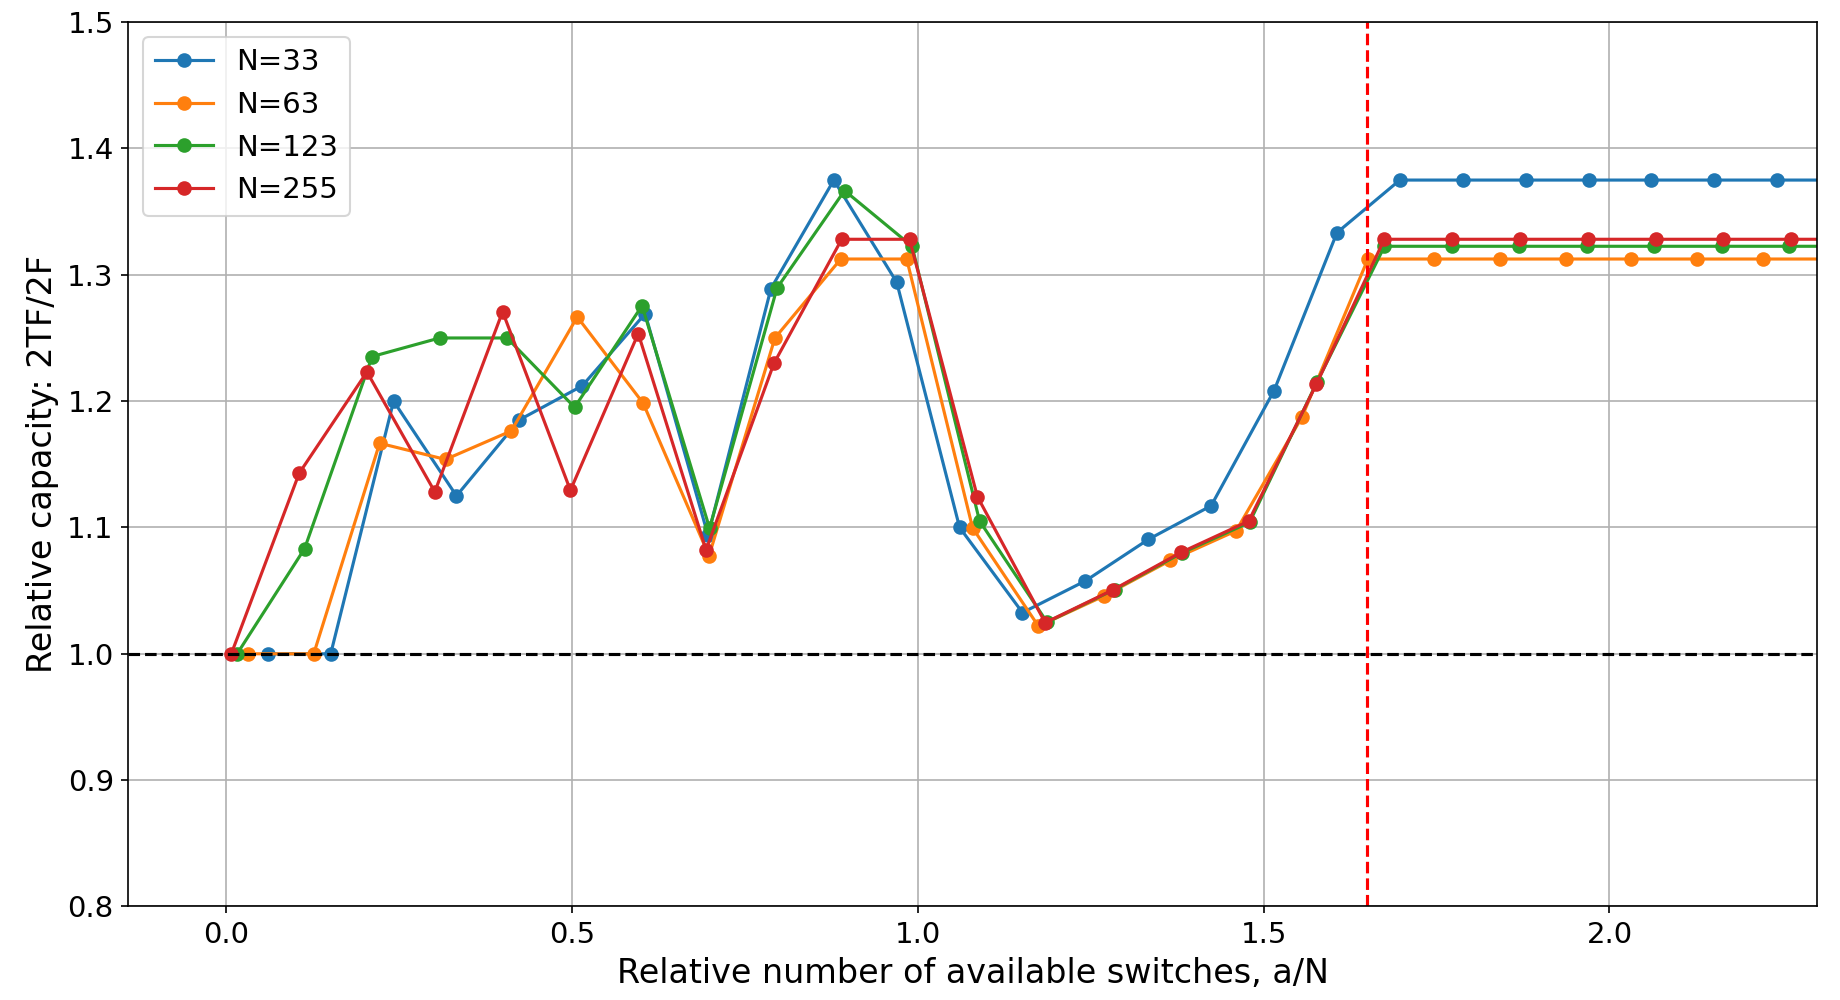
\includegraphics[width=0.8\linewidth]{compare_relative_2f_2.png}
\end{figure}

\noindent ・Theorem 4について, $N=128, 256$($N>120$)のとき, $1.66 \leq \frac{a}{N}$であれば, $f_{2TF}(a; N) > 1.3f_{2F}(a; N)$を満たすはず. 
実際にグラフより, この区間で$30\%$以上の増加が見られた(赤のライン以降).\\
・Theorem 1について, $N \pmod{6}$の値に関係なく, $f_{2F}(a; N) \leq f_{2TF}(a; N)$が成り立つ($y=1$より大きい)ことがグラフより確認できた. 

\subsection{最大・最小・平均スイッチング容量}
・2TF/3UFのRelative switching capacity
\begin{figure}[H]
  \centering
  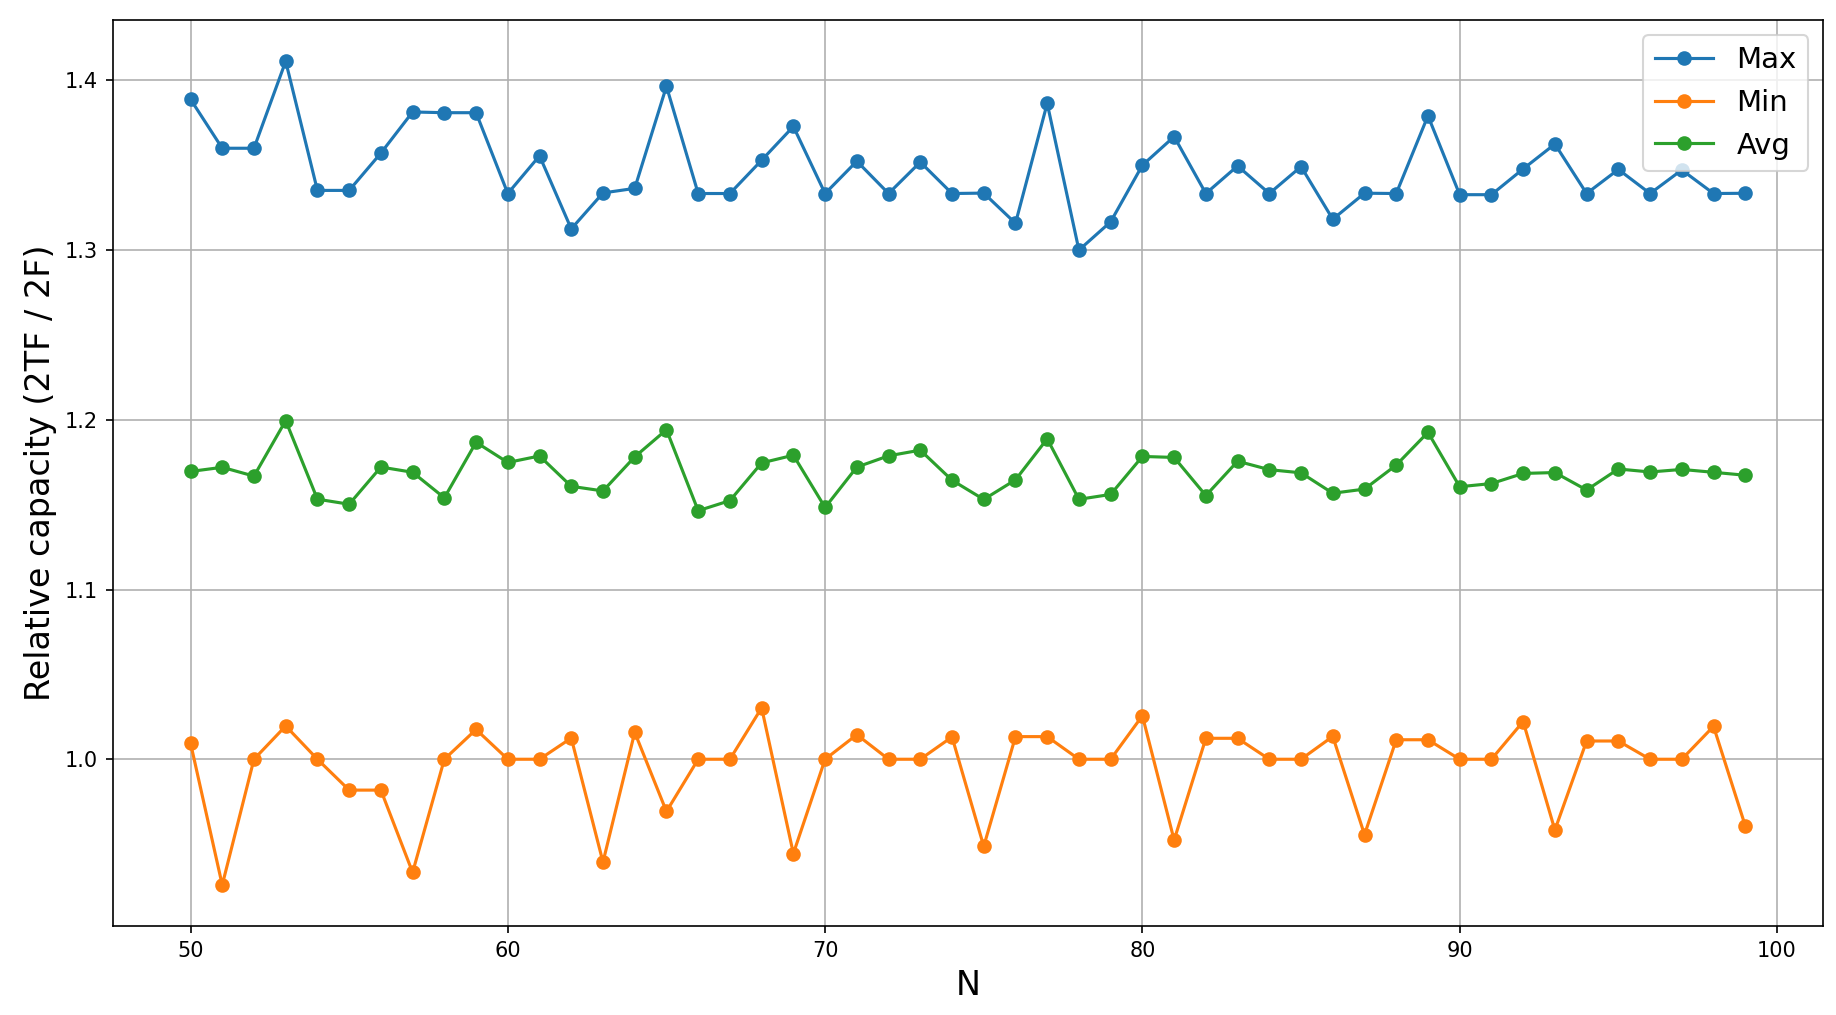
\includegraphics[width=0.8\linewidth]{maxmin_capacity_3uf.png}
\end{figure}

\noindent →2TFは3UFに比べて, 平均約$17\%$, 最大約$35\%$のスイッチング容量の増加が確認できた.\\
→Capacity Reversingも確認できる. \\

・2TF/2FのRelative switching capacity
\begin{figure}[H]
  \centering
  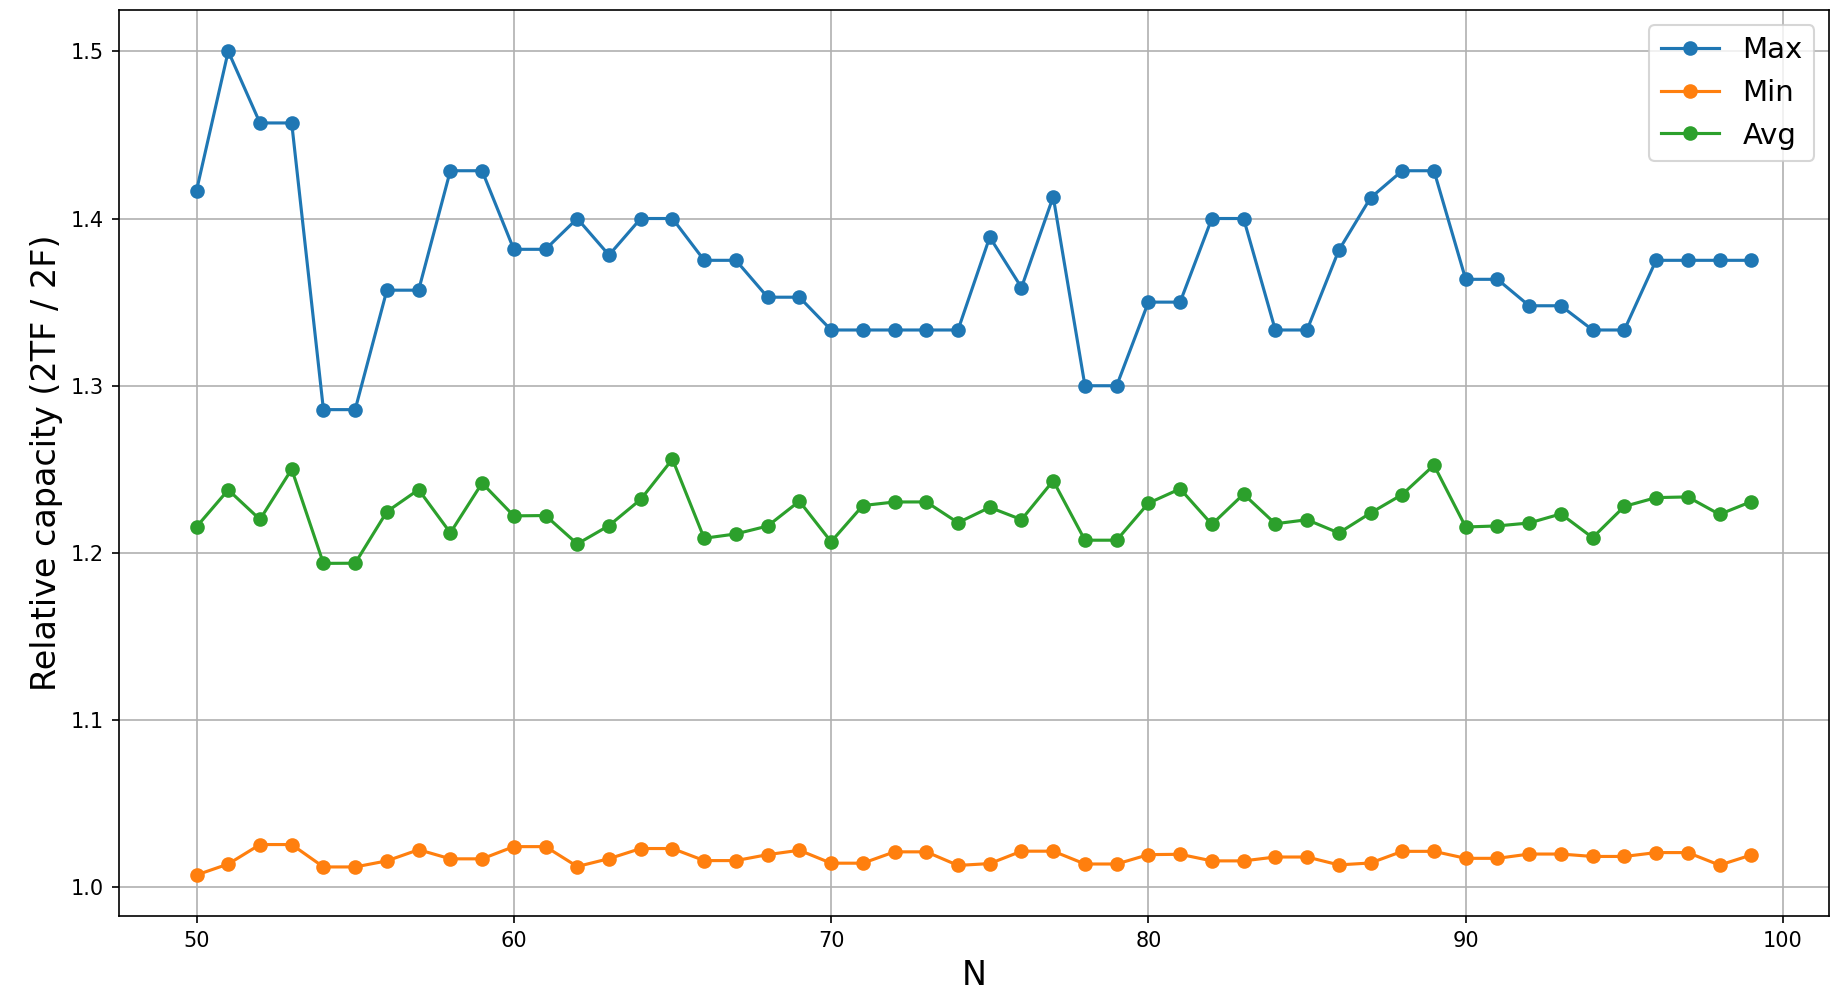
\includegraphics[width=0.8\linewidth]{maxmin_capacity_2f.png}
\end{figure}

→2TFは2Fに比べて, 平均約$21\%$, 最大約$40\%$のスイッチング容量の増加が確認できた.


\subsection{Capacity Reversingの分析(3UF-2TF)}
\begin{figure}[H]
  \centering
  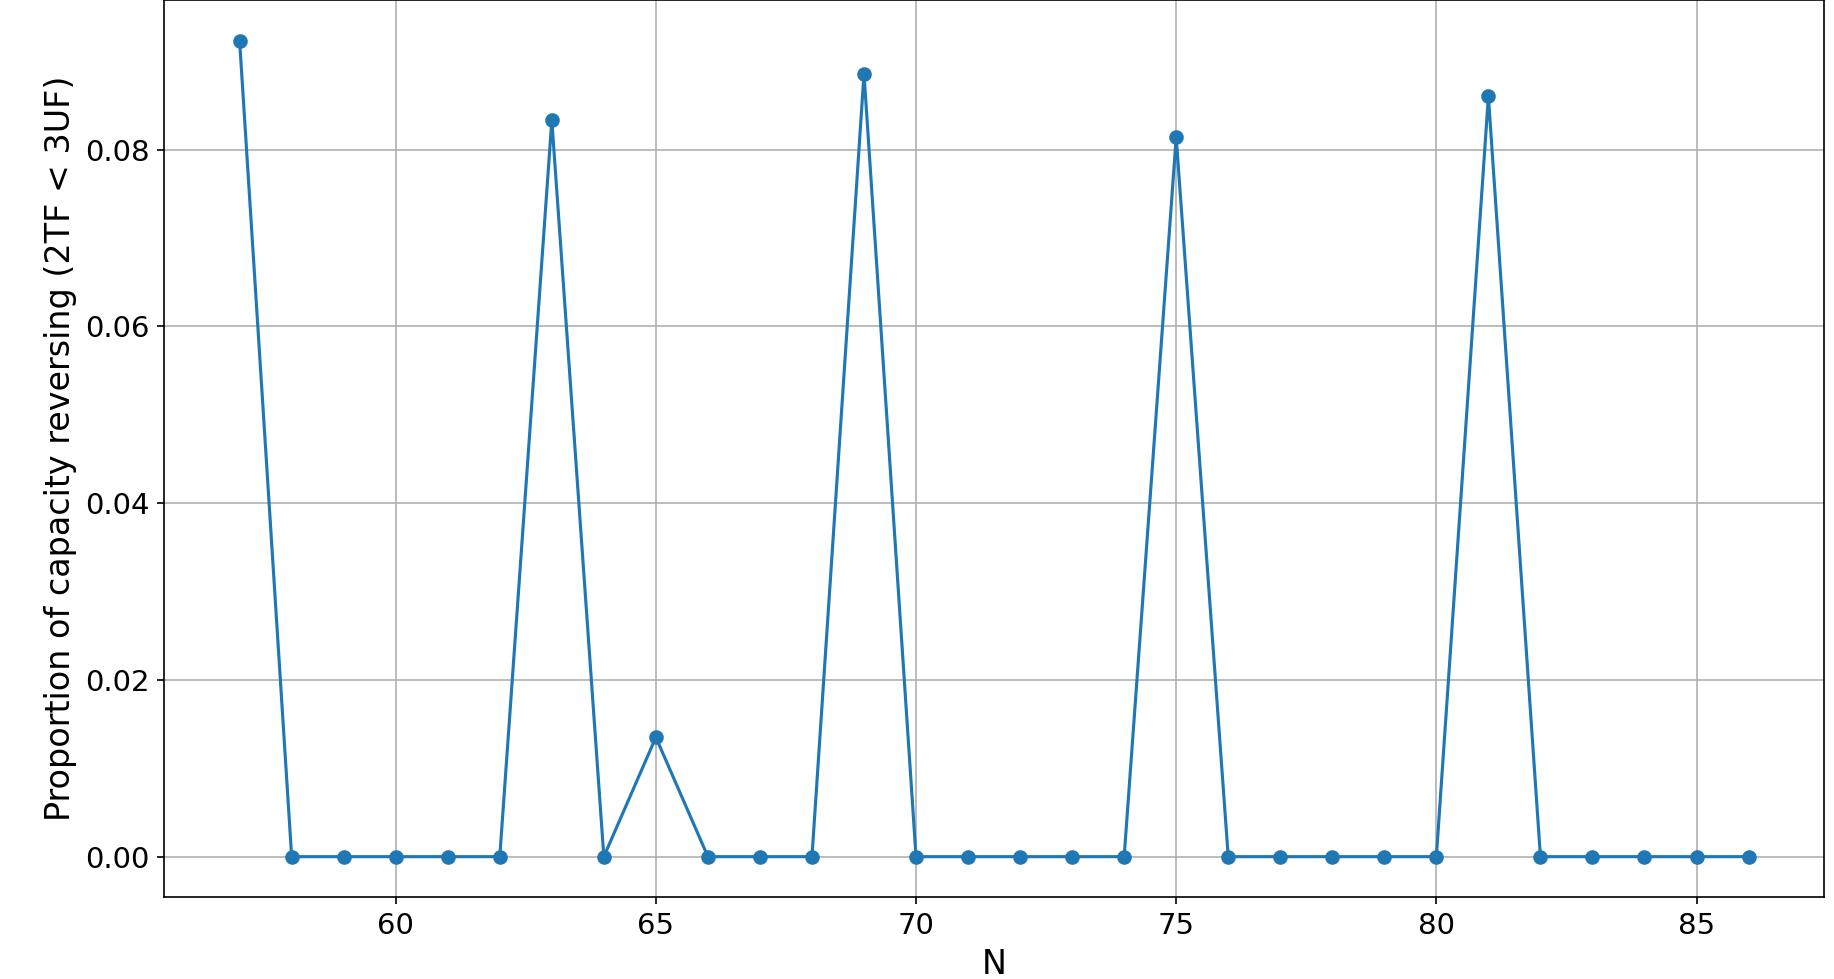
\includegraphics[width=0.8\linewidth]{capacity_reversing_1.png}
\end{figure}

\noindent ・山(0→0.08)の間隔は6→$N \equiv 3 \pmod{6}$に対応. \\



\end{document}